%!TEX program = xelatex
\documentclass[dvipsnames, svgnames,a4paper,11pt]{article}
% ----------------------------------------------------
%   中山大学物理与天文学院本科实验报告模板
%   作者:Huanyu Shi,2019级
%   知乎:https://www.zhihu.com/people/za-ran-zhu-fu-liu-xing
%   Github:https://github.com/Huanyu-Shi/SYSU-SPA-Labreport-Template
%   Last update : 2023.4.10
% ----------------------------------------------------

% ----------------------------------------------------- 
%	加边框的命令
%	参考:https://tex.stackexchange.com/questions/531559/how-to-add-the-page-border-for-first-two-pages-in-latex
\usepackage{tikz}
\usetikzlibrary{calc}
\usepackage{eso-pic}
\AddToShipoutPictureBG{%
\begin{tikzpicture}[overlay,remember picture]
\draw[line width=0.6pt] % 边框粗细
    ($ (current page.north west) + (0.6cm,-0.6cm) $)
    rectangle
    ($ (current page.south east) + (-0.6cm,0.6cm) $); % 边框位置
\end{tikzpicture}}


\usepackage{xcolor}
\definecolor{c1}{HTML}{2752C9} % 目录颜色
\definecolor{c2}{RGB}{190,20,83} % 引用颜色

\usepackage{ctex}
\usepackage[top=28mm,bottom=28mm,left=15mm,right=15mm]{geometry}
\usepackage{hyperref} 
\hypersetup{
	colorlinks,
	linktoc = section, % 超链接位置,选项有section, page, all
	linkcolor = c1, % linkcolor 目录颜色
	citecolor = c1  % citecolor 引用颜色
}
\usepackage{amsmath,enumerate,multirow,float}
\usepackage{tabularx}
\usepackage{tabu}
\usepackage{subfig}
\usepackage{fancyhdr}
\usepackage{graphicx}
\usepackage{wrapfig}  
\usepackage{physics}
\usepackage{appendix}
\usepackage{amsfonts}

%
\usepackage{tcolorbox}
\tcbuselibrary{skins,breakable}
\newtcolorbox{tbox}[2][]{
    colframe=black!70!,
    breakable,
    enhanced,
	boxrule =0.5pt,
    title = {#2},
    fonttitle = \large\kaishu\bfseries,
	drop fuzzy shadow,
    #1
}
\newtcolorbox[auto counter,number within=section]{question}[1][]{
  top=2pt,bottom=2pt,arc=1mm,
  boxrule=0.5pt,
%   frame hidden,
  breakable,
  enhanced, %跨页后不会显示下边框
  coltitle=c1!80!gray,
  colframe=c1,
  colback=c1!3!white,
  drop fuzzy shadow,
  title={思考题~\thetcbcounter:\quad},
  fonttitle=\bfseries,
  attach title to upper,
  #1
}
\newcommand{\setLhead}[1]{%
  \lhead{{\color{gray}\kaishu #1}} % 定义新的命令,设置右边页眉的内容
}
\newcommand{\setRhead}[1]{%
  \rhead{{\color{gray}\kaishu #1}} % 定义新的命令,设置右边页眉的内容
}
% ---------------------------------------------------------------------
%	利用cleveref改变引用格式,\cref是引用命令
\usepackage{cleveref}
\crefformat{figure}{#2{\textcolor{c2}{图 #1}}#3} % 图片的引用格式
\crefformat{equation}{#2{(\textcolor{c2}{#1})}#3} % 公式的引用格式
\crefformat{table}{#2{\textcolor{c2}{表 #1}}#3} % 表格的引用格式


% ---------------------------------------------------------------------
%	页眉页脚设置
\fancypagestyle{plain}{\pagestyle{fancy}}
\pagestyle{fancy}
\setLhead{中山大学物理与天文学院基础物理实验预习报告}
%\lhead{\kaishu 中山大学物理与天文学院物理实验\uppercase\expandafter{\romannumeral3}} % 左边页眉,学院 + 课程
%\rhead{{\color{gray}\kaishu Template 实验报告模板}} % 右边页眉,实验报告标题
\setRhead{实验1\hspace{1pt}冰的熔化热测量}
\cfoot{\thepage} % 页脚,中间添加页码


% ---------------------------------------------------------------------
%	对目录、章节标题的设置
\renewcommand{\contentsname}{\centerline{\huge 目录}}
\usepackage{titlesec}
\usepackage{titletoc}
% \titleformat{章节}[形状]{格式}{标题序号}{序号与标题间距}{标题前命令}[标题后命令]
\titleformat{\section}{\centering\LARGE\songti}{}{1em}{}

% ---------------------------------------------------------------------
%   listing代码环境设置
\usepackage{listings}
\lstloadlanguages{python}
\lstdefinestyle{pythonstyle}{
backgroundcolor=\color{gray!5},
language=python,
frameround=tftt,
frame=shadowbox, 
keepspaces=true,
breaklines,
columns=spaceflexible,                   
basicstyle=\ttfamily\small, % 基本文本设置,字体为teletype,大小为scriptsize
keywordstyle=[1]\color{c1}\bfseries, 
keywordstyle=[2]\color{Red!70!black},   
stringstyle=\color{Purple},       
showstringspaces=false,
commentstyle=\ttfamily\scriptsize\color{green!40!black},%注释文本设置,字体为sf,大小为smaller
tabsize=2,
morekeywords={as},
morekeywords=[2]{np, plt, sp},
numbers=left, % 代码行数
numberstyle=\it\tiny\color{gray}, % 代码行数的数字字体设置
stepnumber=1,
rulesepcolor=\color{gray!30!white}
}




% ---------------------------------------------------------------------
%	其他设置
\def\degree{${}^{\circ}$} % 角度
\graphicspath{{./images/}} % 插入图片的相对路径
\allowdisplaybreaks[4]  %允许公式跨页 % 导入模板的相关设置
\usepackage{lipsum}
\usepackage{indentfirst}
\usepackage{pdfpages}
\usepackage{multirow}
\usepackage{subfig}
\usepackage{graphicx}
\usepackage{float} 
\usepackage{booktabs}
\usepackage{enumerate}
\renewcommand{\d}{\mathrm{d}}


%---------------------------------------------------------------------
%	正文
%---------------------------------------------------------------------
\setRhead{多普勒效应综合实验}%实验名称
\begin{document}


\begin{table}
	\renewcommand\arraystretch{1.7}
	\begin{tabularx}{\textwidth}{
		|X|X|X|X
		|X|X|X|X|}
	\hline
	\multicolumn{2}{|c|}{预习报告}&\multicolumn{2}{|c|}{实验记录}&\multicolumn{2}{|c|}{分析讨论}&\multicolumn{2}{|c|}{总成绩}\\
	\hline
	 & &  & &  & &  & \\
	\hline
	\end{tabularx}
\end{table}


\begin{table}
	\renewcommand\arraystretch{1.7}
	\begin{tabularx}{\textwidth}{|X|X|X|X|}
	\hline
	专业:& 物理学类 &年级:& 2023级\\
	\hline
	姓名:& 姚昊廷  & 学号:&22322091\\
	\hline
	实验时间:& 2024.11.21& 教师签名:& \\
	\hline
	\end{tabularx}
\end{table}

\begin{center}
	\LARGE 多普勒效应综合实验
\end{center}

\textbf{【实验报告注意事项】}
\begin{enumerate}
	\item 实验报告由三部分组成:
	\begin{enumerate}
		\item 预习报告:(提前一周)认真研读\underline{\textbf{实验讲义}},弄清实验原理;实验所需的仪器设备、用具及其使用(强烈建议到实验室预习),完成课前预习思考题;了解实验需要测量的物理量,并根据要求提前准备实验记录表格(第一循环实验已由教师提供模板,可以打印)。预习成绩低于10分(共20分)者不能做实验。
	    \item 实验记录:认真、客观记录实验条件、实验过程中的现象以及数据。实验记录请用珠笔或者钢笔书写并签名(\textcolor{red}{\textbf{用铅笔记录的被认为无效}})。\textcolor{red}{\textbf{保持原始记录,包括写错删除部分,如因误记需要修改记录,必须按规范修改。}}(不得输入电脑打印,但可扫描手记后打印扫描件);离开前请实验教师检查记录并签名。
	    \item 分析讨论:处理实验原始数据(学习仪器使用类型的实验除外),对数据的可靠性和合理性进行分析;按规范呈现数据和结果(图、表),包括数据、图表按顺序编号及其引用;分析物理现象(含回答实验思考题,写出问题思考过程,必要时按规范引用数据);最后得出结论。
	\end{enumerate}
	\textbf{实验报告就是将预习报告、实验记录、和数据处理与分析合起来,加上本页封面。}
	\item 每次完成实验后的一周内交\textbf{实验报告}(特殊情况不能超过两周)。
	\item 除实验记录外,实验报告其他部分建议双面打印。
\end{enumerate}

{\textbf{【实验安全与实验室注意事项】}\\
一、验证多普勒效应实验设备安装时注意事项:
\begin{enumerate}
	\item 安装时要尽量保证红外接收器、小车上的红外发射器和超声接收器、超声发射器三者之间在同一轴线上,以保证信号传输良好;
	\item 安装时不可挤压连接电缆,以免导线折断;
	\item 安装时请确认橡胶圈是否套在主动轮上;
	\item 小车不使用时应立放,避免小车滚轮沾上污物,影响实验进行。
\end{enumerate}}
\noindent 二、研究自由落体运动设备安装时注意事项:
\begin{enumerate}
    \item 须将“自由落体接收器保护盒”套于发射器上,避免发射器在非正常操作时受到冲击而损坏;
    \item 安装时切不可挤压电磁阀上的电缆。
\end{enumerate}

\clearpage
\tableofcontents
\clearpage

\setcounter{section}{0}
\section{多普勒效应综合实验\ \textbf{预习报告}}
	
\subsection{实验目的}
\begin{enumerate}
    \item 测量超声接收器运动速度与接收频率之间的关系,验证多普勒效应,并由f-V 关系直线的斜率
	求声速。
	\item 利用多普勒效应测量物体运动过程中多个时间点的速度,查看V-t 关系曲线,或调阅有关测量
	数据,即可得出物体在运动过程中的速度变化情况,可研究:
	\begin{enumerate}[1)]
		\item 自由落体运动,并由V-t 关系直线的斜率求重力加速度。
		\item 简谐振动,可测量简谐振动的周期等参数,并与理论值比较。
		\item 匀加速直线运动,测量力、质量与加速度之间的关系,验证牛顿第二定律。
		\item 其它变速直线运动。
	\end{enumerate}
\end{enumerate}
\subsection{仪器用具}
\begin{table}[htbp]
	\centering
	\renewcommand\arraystretch{1.6}
	% \setlength{\tabcolsep}{10mm}
	\begin{tabular}{p{0.05\textwidth}|p{0.20\textwidth}|p{0.05\textwidth}|p{0.5\textwidth}}
	\hline
	编号& 仪器用具名称 & 数量 &  主要参数(型号,测量范围,测量精度等) \\
	\hline
	1&多普勒效应综合实验仪&1 &ZKY-DPL-3\\
	\hline
	2&超声发射/接收器 &1&谐振频率40000-1000Hz\\
	\hline
	3&红外发射/接收器&2&\\
	\hline
	4&导轨&1&\\
	\hline
	5&运动小车、支架、光电门、电
	磁铁、弹簧、滑轮、砝码及电
	机控制器等组成。&1&\\
	\hline
\end{tabular}
\end{table}

\textbf{【原理概述】}\\
\begin{question}
	解释超声的多普勒效应
	\tcblower
	我们假设发射器A与接收器B的时间是一致的,由于声速有限且AB间距在变化。为简化模型我们设声波为单频
	$f$。那么B相对A的滞后量$\Delta \varphi=\frac{2\pi d_{AB}f}{c}$随时间改变,那么B接收到的频率为$f-\frac{1}{2\pi}\frac{\d\Delta \varphi}{\d t}\neq f$
	即接收频率与发射频率发生了偏差。
\end{question}

\begin{question}
	简述为什么选择超声的红外调制与接收
	\tcblower
	使用超声与红外都是人耳/眼无法接收的信号,可避免仪器对人感官的直接刺激。超声避开了人发出声音的频段
	减少实验中人为干扰且穿透力较高可减少不同实验小组之间的影响实验对环境的噪声污染,红外光能量较低强度不高
	不易损伤人体。
\end{question}

\begin{question}
	简述验证多普勒效应并由测量数据计算声速的方法及步骤
	\tcblower
	固定发射频率$f_0$多次改变小车速率$v$测出接收频率$f$,算出$f-v$图中回归直线斜率以此验证多普勒效应
	回归直线截距可表示声速测量值。
\end{question}

\begin{question}
	简述研究自由落体运动,求自由落体加速度的方法及步骤
	\tcblower
	固定发射器使接收器自由落体利用多普勒效应测量下落过程中时间$t$与速度$v$的值,作出$v-t$图,$v-t$图中回归直线斜率
	即为重力加速度。
\end{question}

\begin{question}
	简述研究简谐振动的方法及步骤
	\tcblower
	固定发射器使接收器自由落体利用多普勒效应测量下落过程中时间$t$与速度$v$的值,作出$v-t$图,取
	$v$第1,11次达到最大值的时间(十个周期)即可计算出$\omega$再与理论值$\omega=\sqrt{\frac{k}{m}}$比较。
\end{question}
\textbf{【实验前思考题】}\\
\begin{question}
	用多普勒效应来\textbf{解释}你生活中遇到的一些现象。
	\tcblower
	站在火车站台上时,驶过的火车鸣笛音调会先变高,后变低。火车接近时,发出的声波频率因相对运动而增加,听起来更尖锐。火车远离时,频率减小,音调变低。
\end{question}


\clearpage
\setLhead{中山大学物理与天文学院基础物理实验记录}
\begin{table}
	\renewcommand\arraystretch{1.7}
	\centering
	\begin{tabularx}{\textwidth}{|X|X|X|X|}
	\hline
	专业:& 物理学类 &年级:& 2023级 \\
	\hline
	姓名: &姚昊廷& 学号:&22322091  \\
	\hline
	室温:&22.0$^\circ$C&实验地点:&A511\ D6\\
	\hline
	学生签名:& & 评分: &\\
	\hline
	实验时间:& 2024.11.21& 教师签名:&\\
	\hline
	\end{tabularx}
\end{table}
\section{多普勒效应综合实验\ \textbf{实验记录}}
\subsection{实验内容、步骤、结果}
\subsubsection{验证多普勒效应并由测量数据计算声速}
\noindent1.简述本次实验方法及过程\\
让小车以不同速度通过光电门,仪器自动记录小车通过光电门时的平均运动速度及与之对应的平均接收频
率。\\
\noindent2.实验数据记录
\begin{table}[H]
	\centering
	\caption{多普勒效应的验证与声速的测量\hfill$T_c=22^\circ$C\ \ \ \ $f_0=40001$Hz}
	\begin{tabularx}{\textwidth}{|X|X|X|X|X|X|}
		\hline
		\multicolumn{6}{|c|}{测量数据}\\
		\hline
		次数i&1&2&3&4&5\\
		\hline
		$v_i$(m/s)&1.12&0.99&0.85&0.71&0.56\\
		\hline
		$f_i$(Hz)&40130&40115&40099&40083&40066\\
		\hline
	\end{tabularx}
\end{table}
\noindent3.实验现象描述\\
固定$f_0$时,当接收器与发射器径向靠近,相对速度越大,接收频率越高。

\subsubsection{研究自由落体运动,求自由落体加速度}
\noindent1.简述本次实验方法及过程\\
让带有超声接收器的接收组件自由下落,利用多普勒效应测量物体运动过程中多个时间点的速度,查看V-t
关系曲线,并调阅有关测量数据,即可得出物体在运动过程中的速度变化情况,进而计算自由落体加速度。\\
\noindent2.实验数据记录
\begin{table}[H]
	\centering
	\caption{自由落体运动的测量($t_{1i}\neq t_{2i}\neq t_{3i}\neq t_{4i}$)}
	\begin{tabularx}{\textwidth}{|X|X|X|X|X|X|X|X|X|X|}
		\hline
		&采样序号i&i=2&i=3&i=4&i=5&i=6&i=7&i=8&i=9\\
		\hline
		\multirow{2}{*}{第一组}&$t_{1i}$/s&0.03&0.06&0.09&0.12&0.15&0.18&0.21&0.24\\
		\cline{2-10}
		&$v_{1i}$&0.57&0.71&1.08&1.36&1.62&1.94&2.20&2.46\\
		\hline
		\multirow{2}{*}{第二组}&$t_{1i}$/s&0.02&0.04&0.06&0.08&0.10&0.12&0.14&0.16\\
		\cline{2-10}
		&$v_{1i}$&0.44&0.58&0.76&0.97&1.15&1.36&1.52&1.76\\
		\hline
		\multirow{2}{*}{第三组}&$t_{1i}$/s&0.015&0.03&0.045&0.06&0.075&0.09&0.105&0.12\\
		\cline{2-10}
		&$v_{1i}$&0.32&0.43&0.53&0.79&0.94&1.04&1.20&1.37\\
		\hline
		\multirow{2}{*}{第四组}&$t_{1i}$/s&0.025&0.05&0.075&0.10&0.125&0.150&0.175&0.20\\
		\cline{2-10}
		&$v_{1i}$&0.32&0.60&0.88&1.16&1.39&1.66&1.88&2.13\\
		\hline
	\end{tabularx}
\end{table}
\noindent3.实验现象描述\\
$vt$基本成线性关系。

\subsubsection{研究简谐振动}
\noindent1.简述本次实验方法及过程\\
使用上一个实验自由落体时使用的竖直导轨,将测量点数与间隔调整至总时间大于10个周期,先使重物开始振动,再开始测量。\\
\noindent2.实验数据记录
\begin{table}[H]
	\centering
	\caption{简谐振动的测量\hfill$M=0.10224$kg\ \ \ \ $m=0.08407$kg}
	\begin{tabularx}{\textwidth}{|X|X|X|}
		\hline
		$\Delta x$(m)&$N_{1max}$(number)&$N_{11max}$(number)\\
		\hline
		0.2541&8&121\\
		\hline
	\end{tabularx}
\end{table}
\noindent3.实验现象描述\\
周期较为均匀,约为10个数据点达到一组极大值。最大值在10个周期中由0.93衰减为0.88。

\subsubsection{研究匀变速直线运动,验证牛顿第二运动定律}
\noindent1.简述本次实验方法及过程\\
滑轮一端悬挂砝码及砝码托,一端悬挂接收器,确保砝码及砝码托质量小于接收器。设置时间间隔及组数使得接收器在15-25个
时间间隔内落地。记录v-t数据和重物质量重复多组实验。\\
\noindent2.实验数据记录
\begin{table}[H]
    \centering
    \caption{匀变速直线运动的测量 \hfill $C=0.07$\quad $J/R^2=0.014$ kg}
    \begin{tabularx}{\textwidth}{|c|c|*{13}{X|}}
        \hline
        \multicolumn{2}{|c|}{采样序号 \(i\)} & 2 & 3 & 4 & 5 & 6 & 7 & 8 & 9 & 10 & 11 & 12 & 13 & 14 \\
        \hline
        \multicolumn{2}{|c|}{$t_i$ (s)} & 0.1 & 0.2 & 0.3 & 0.4 & 0.5 & 0.6 & 0.7 & 0.8 & 0.9 & 1.0 & 1.1 & 1.2 & 1.3 \\
        \hline
        $M_1=$ 0.08077 kg & $v_{1i}$ (m/s) & 0.20 & 0.28 & 0.36 & 0.43 & 0.53 & 0.60 & 0.71 & 0.76 & 0.85 & 0.95 & 1.02 & 1.09 & 1.16 \\
        \hline
        $M_2=$ 0.09277 kg & $v_{2i}$ (m/s) & 0.06 & 0.09 & 0.09 & 0.13 & 0.16 & 0.18 & 0.20 & 0.21 & 0.23 & 0.25 & 0.27 & 0.30 & 0.32 \\
        \hline
		\multicolumn{2}{|c|}{$t_i$}&0.03&0.06&0.09&0.12&0.15&0.18&0.21&0.24&0.27&0.3&0.33&0.36&0.39\\
		\hline
        $M_3=$ 0.04468 kg & $v_{3i}$ (m/s) & 0.23 & 0.36 & 0.46 & 0.57 & 0.64 & 0.74 & 0.86 & 0.95 & 1.08 & 1.15 & 1.23 & 1.34 & 1.43 \\
        \hline
        $M_4=$ 0.05621 kg & $v_{4i}$ (m/s) & 0.20 & 0.27 & 0.34 & 0.43 & 0.50 & 0.53 & 0.64 & 0.69 & 0.76 & 0.85 & 0.90 & 0.97 & 1.08 \\
        \hline
    \end{tabularx}
\end{table}
\noindent3.实验现象描述\\
$vt$基本成线性关系。

\subsection{实验过程中遇到的问题记录}
实验一中小车初始没电,导致第一次实验时数据出现明显错误。


\clearpage
\setLhead{中山大学物理与天文学院基础物理实验分析与讨论}
\begin{table}
	\renewcommand\arraystretch{1.7}
	\begin{tabularx}{\textwidth}{|X|X|X|X|}
	\hline
	专业:& 物理学 &年级:& 2023级\\
	\hline
	姓名: &姚昊廷& 学号:&22322091 \\
	\hline
    日期:&2024.11.21 & 评分: &\\
	\hline
	\end{tabularx}
\end{table}

\section{多普勒效应综合实验\ \textbf{分析与讨论}}
\subsection{验证多普勒效应并由测量数据计算声速}
\subsubsection*{实验数据处理}
\noindent 根据原始测量数据,做出f-v曲线。
\begin{figure}[H]
	\centering
	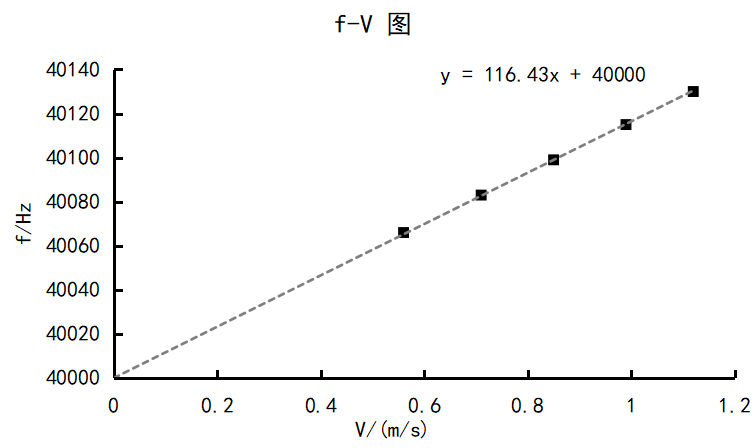
\includegraphics[width=\textwidth]{多普勒fv图png.png}
\end{figure}
\subsubsection*{实验结果计算:}
\noindent 计算直线斜率$k$ (1/m)和声速测量值$u=f_0/k$ (m/s)。\\
$$k=116.43m^{-1},u=\frac{f_0}{k}=343.55\text{m/s}$$
\subsubsection*{实验数据分析}
\noindent 将计算值与声速理论值进行比较,分析误差。\\
$$u_0=331\sqrt{1+\frac{t_c}{273}}|_{t_c=22^\circ\text{C}}=344.08\text{m/s},\eta=\frac{u_0-u}{u}=0.15\%$$
误差太小,难以进一步判断分析误差来源,可能与空气与理想气体差别引起。

\subsection{研究自由落体运动,求自由落体加速度}
\subsubsection*{实验数据处理}
\noindent 根据上表原始测量数据,计算重力加速度的值。\\
经过回归计算得
\begin{table}[H]
	\centering
	\begin{tabularx}{0.8\textwidth}{|c|c|c|}
		\cline{1-3}
		测量序号i&线性回归斜率$k_i$(m/s$^2$)&相关系数$r_i$\\
		\cline{1-3}
		1&9.33&0.998\\
		\cline{1-3}
		2&9.48&0.999\\
		\cline{1-3}
		3&10.22&0.996\\
		\cline{1-3}
		4&10.30&0.999\\
		\cline{1-3}
	\end{tabularx}
\end{table}
平均重力加速度为$\overline{g}=9.8325$m/s$^2$。
\subsubsection*{实验数据分析}
\noindent 实验数据分析,将实验计算值与当地的重力加速度理论值进行比较,进行误差分析。\\
查阅资料得到广州重力加速度为$g=9.7833$m/s$^2$。
$$\eta=\frac{\overline{g}-g}{g}=0.05\%$$
测得值偏大但误差较小,可认为是仪器老化导致测量精度问题引起。

\subsection{研究简谐振动}
\subsubsection*{实验数据处理与结果表达}
\noindent (1)根据原始测量数据,计算弹簧的振动角频率$\omega=\frac{2\pi}{T}$\\
$$T=\frac{1}{10}(N_{11max}-N_{1max})\Delta t=1.13\text{s},\omega=5.56\text{rad/s }$$
(2)根据弹簧的参数,计算其固有角频率;\\
$$k=\frac{mg}{\Delta x}=3.2368\text{N/m},\omega_0=\sqrt{\frac{k}{M}}=5.63\text{rad/s }$$
\subsubsection*{实验数据分析}
\noindent 将实验实验测得的角频率数据与理论值比较,分析误差。\\
相对误差为$\eta=\frac{\omega_0-\omega}{\omega}=1.26\%$误差来源可能是弹簧自重和空气阻力未计入。

\subsection{研究匀变速直线运动,验证牛顿第二运动定律}
\subsubsection*{数据处理与结果表达}
\noindent 以实验得出的加速度$a$作纵轴,$[(1-C)M-m]/[(1-C)M+m+J/R^2]$作横轴作图
\begin{table}[H]
	\centering
	\begin{tabularx}{0.8\textwidth}{|c|c|X|}
		\hline
		测量序号i&加速度(线性回归斜率)$a_i$(m/s$^2$)&$[(1-C)M-m]/[(1-C)M+m+J/R^2]$\\
		\hline
		1&0.814&0.076\\
		\hline
		2&0.212&0.012\\
		\hline
		3&3.299&0.328\\
		\hline
		4&2.374&0.236\\
		\hline
	\end{tabularx}
\end{table}
\begin{figure}[H]
	\centering
	\includegraphics[width=\textwidth]{a-xx图.png}
\end{figure}
\subsubsection*{实验数据分析}
\noindent 分析上图中的关系否为线性关系?若是线性关系,求出直线的斜率即重力加速度;本实验中滑轮的摩擦力对实验影响较大,可以从系统误差的角度分析其对测量结果的影响。\\
$R^2=0.99992$十分接近1因此是线性关系,拟合曲线斜率为9.76678,相对误差为
$$\eta=\frac{g-g_0}{g}=-0.17\%$$
误差来源可能有
\begin{enumerate}
	\item $m$的取值过于接近$M$使得$M$下降太慢轮子转速慢,滑轮与轴间的摩擦系数微小各向异性体现出来。
	\item $M$离开电磁铁后仍有剩磁导致干扰实验。
\end{enumerate}

\subsection{实验后思考题}
\begin{question}
	根据上面几个实验内容,参考其测量方法和步骤,以测量的结果与理论值比较,研究物理运动的规律。请学生根据学过的原理自行设计一个实验内容及方案(如研究摩擦力与运动速度的关系,或与摩擦介质的关系)。
	\tcblower
	将实验1中的皮带上加装一个力传感器,并通过电机使得小车匀速在导轨上行驶,利用光电门测出小车此时速度
	并记录此时皮带拉力,因为小车此时水平方向仅受摩擦力与皮带拉力,因此匀速行驶时摩擦力与皮带拉力相等。
	改变小车匀速行驶的速度$v$,记录不同速度下的皮带张力$T$。作出$T-v$图,可知小车所受摩擦力与运动速度的关系。
\end{question}
\clearpage
% ---------------------------------------------------------------------
%   参考文献
%   注:使用参考文献时应按照xelatex->bibtex->xelatex->xelatex顺序进行编译
\phantomsection
%\addcontentsline{toc}{section}{参考文献}
\bibliographystyle{unsrt}
\bibliography{myref}
%\begin{thebibliography}{9}
	%\bibitem{ref1} 凤飞龙,黄育红,金蔚,王公正,崔致远,“外推法计算冰的熔解热的理论依据及Matlab实现方案”,《大学物理》,第42卷,第2期
%\end{thebibliography}


\clearpage
\appendix
\appendixpage
\addappheadtotoc
%\subsection*{相图代码}
%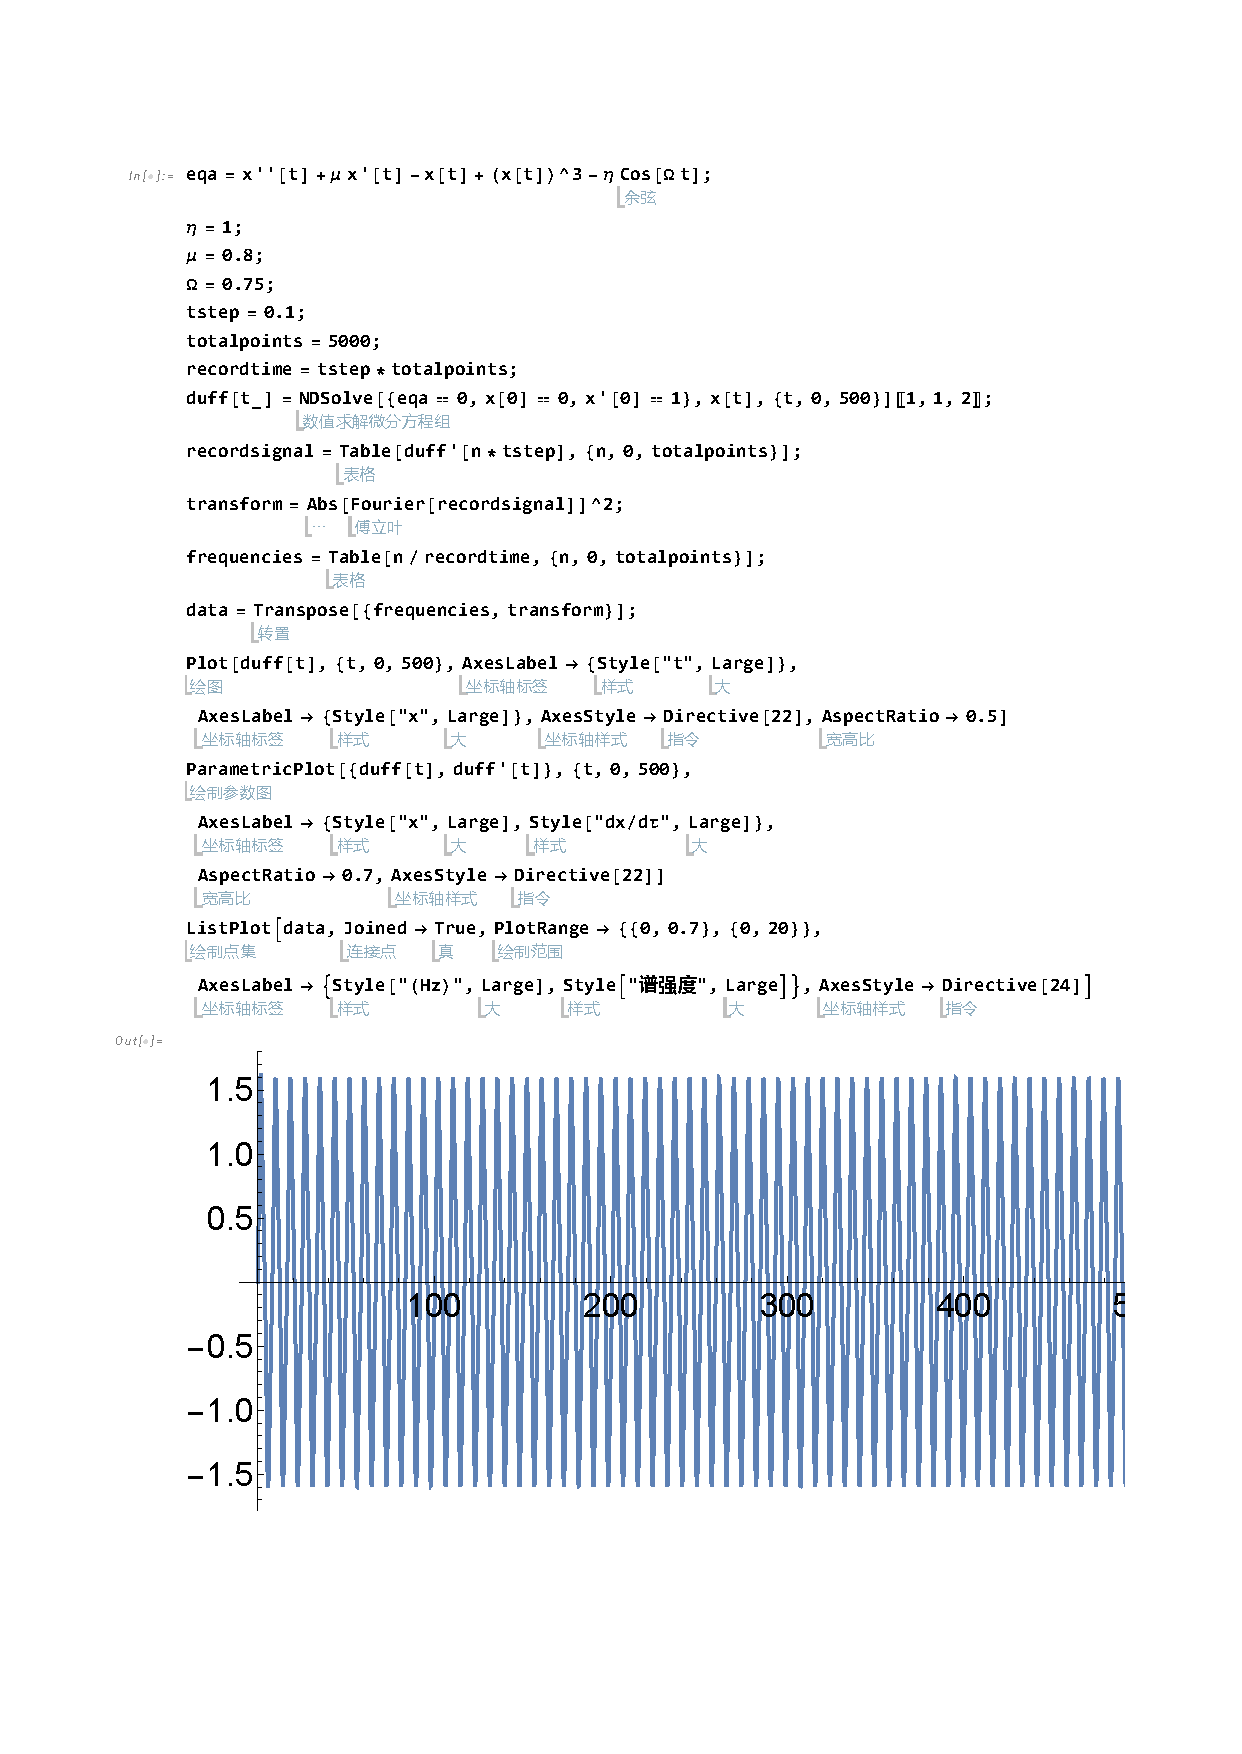
\includepdf[pages=-]{chaos.pdf}
%\subsection*{原件扫描}
%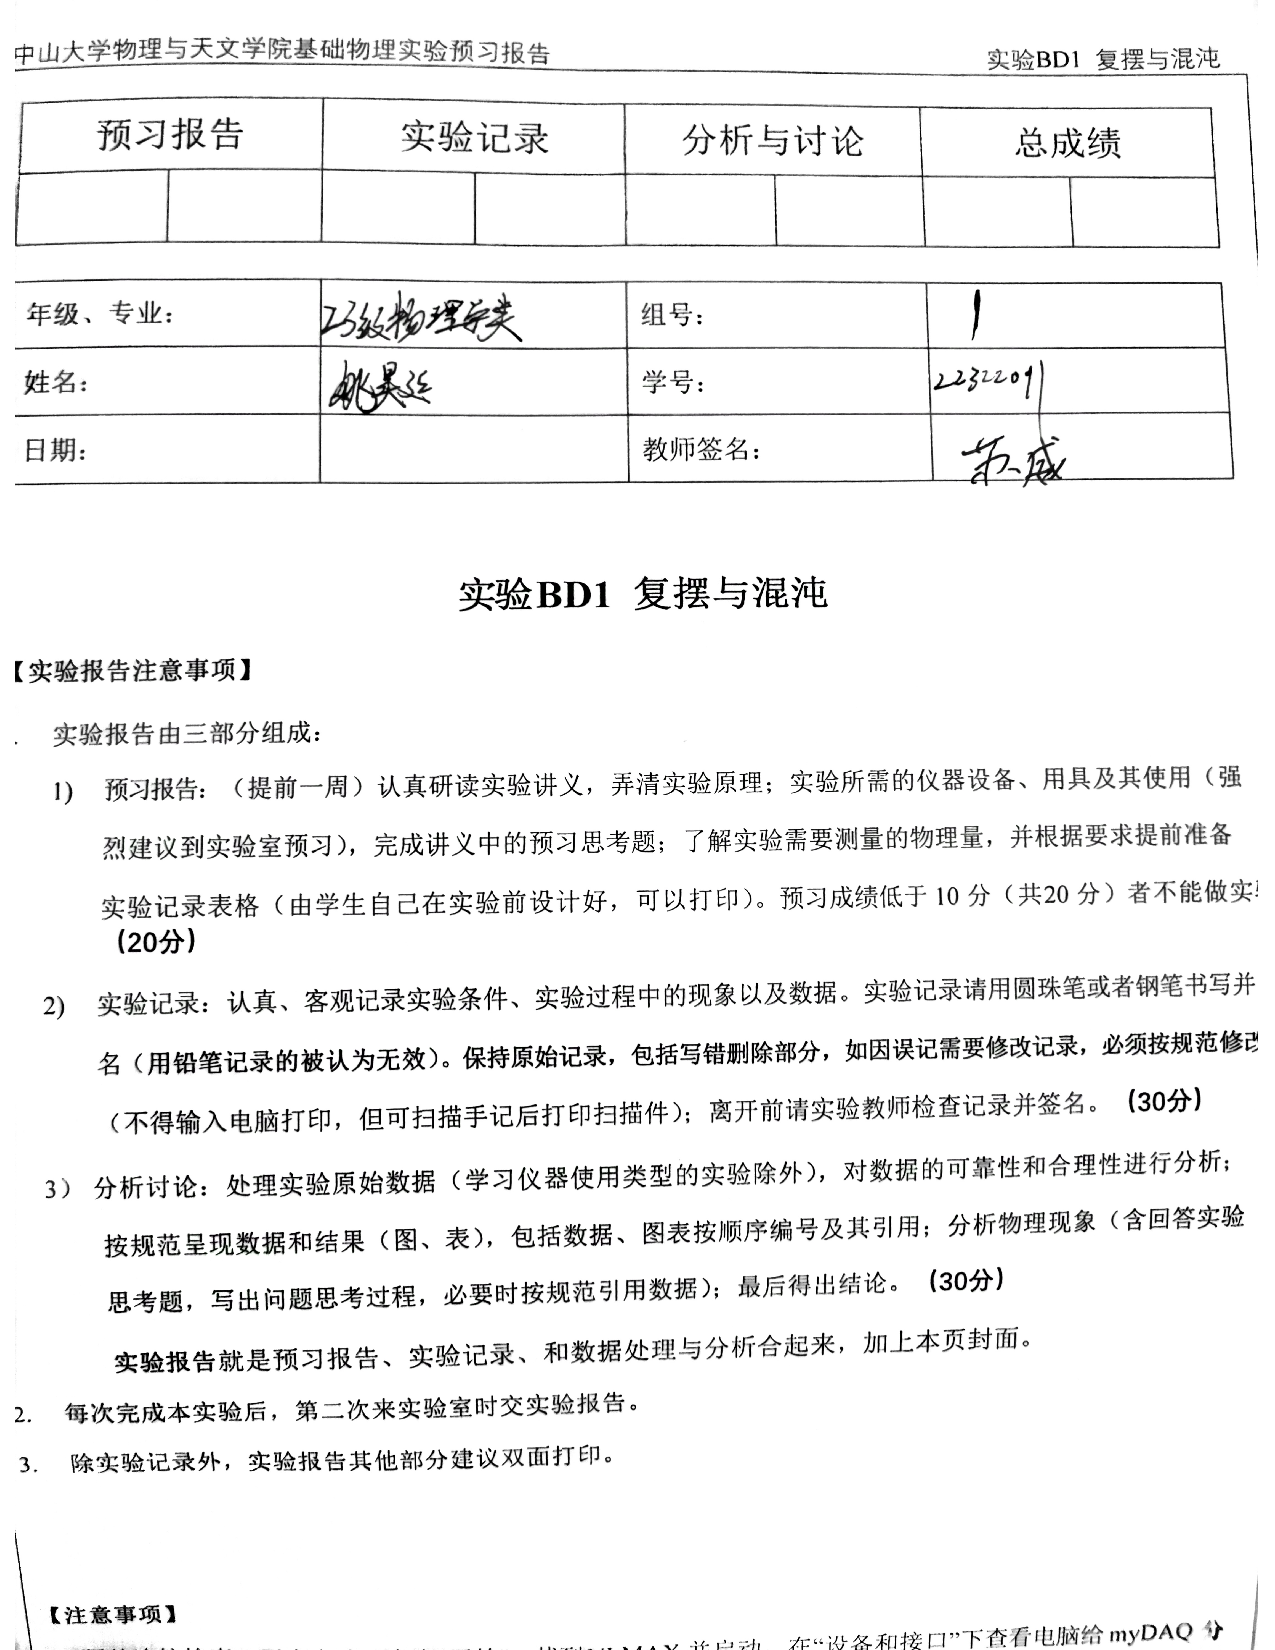
\includepdf[pages=-]{实验3原件.pdf}
\begin{figure}[H]
	\centering
	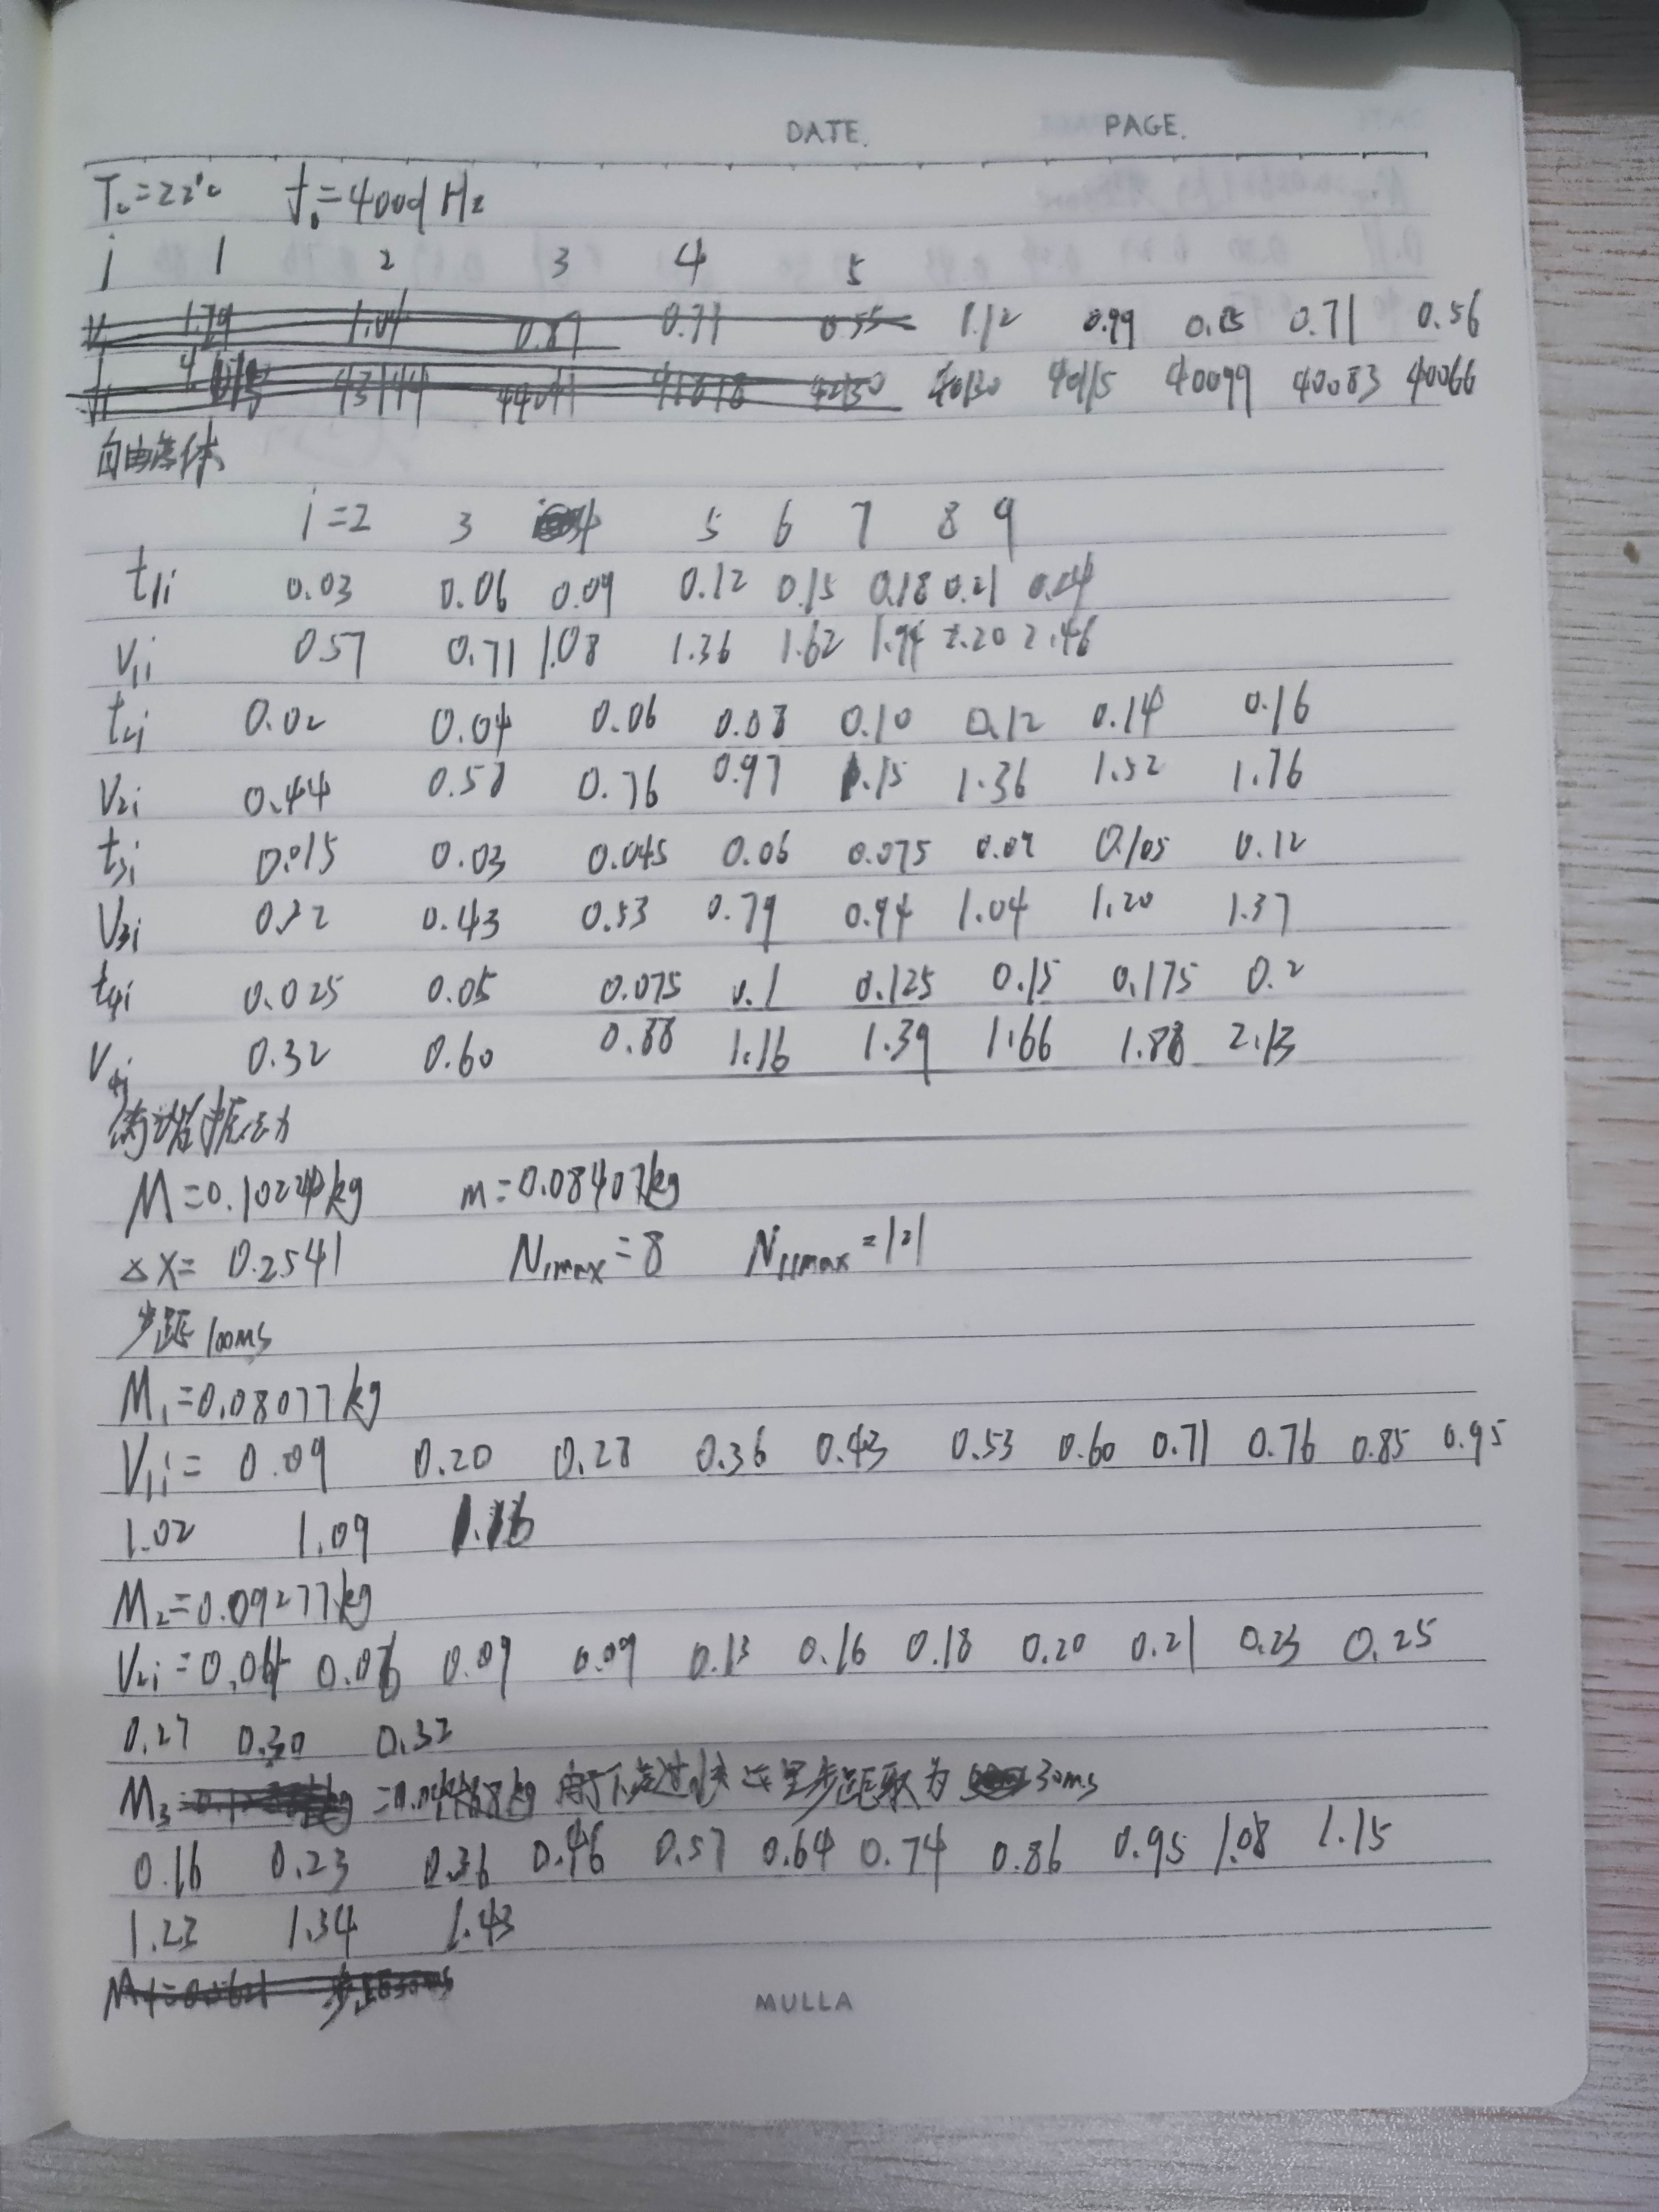
\includegraphics[width=0.4\textwidth]{多普勒原件1.jpg}
\end{figure}

\begin{figure}[H]
	\centering
	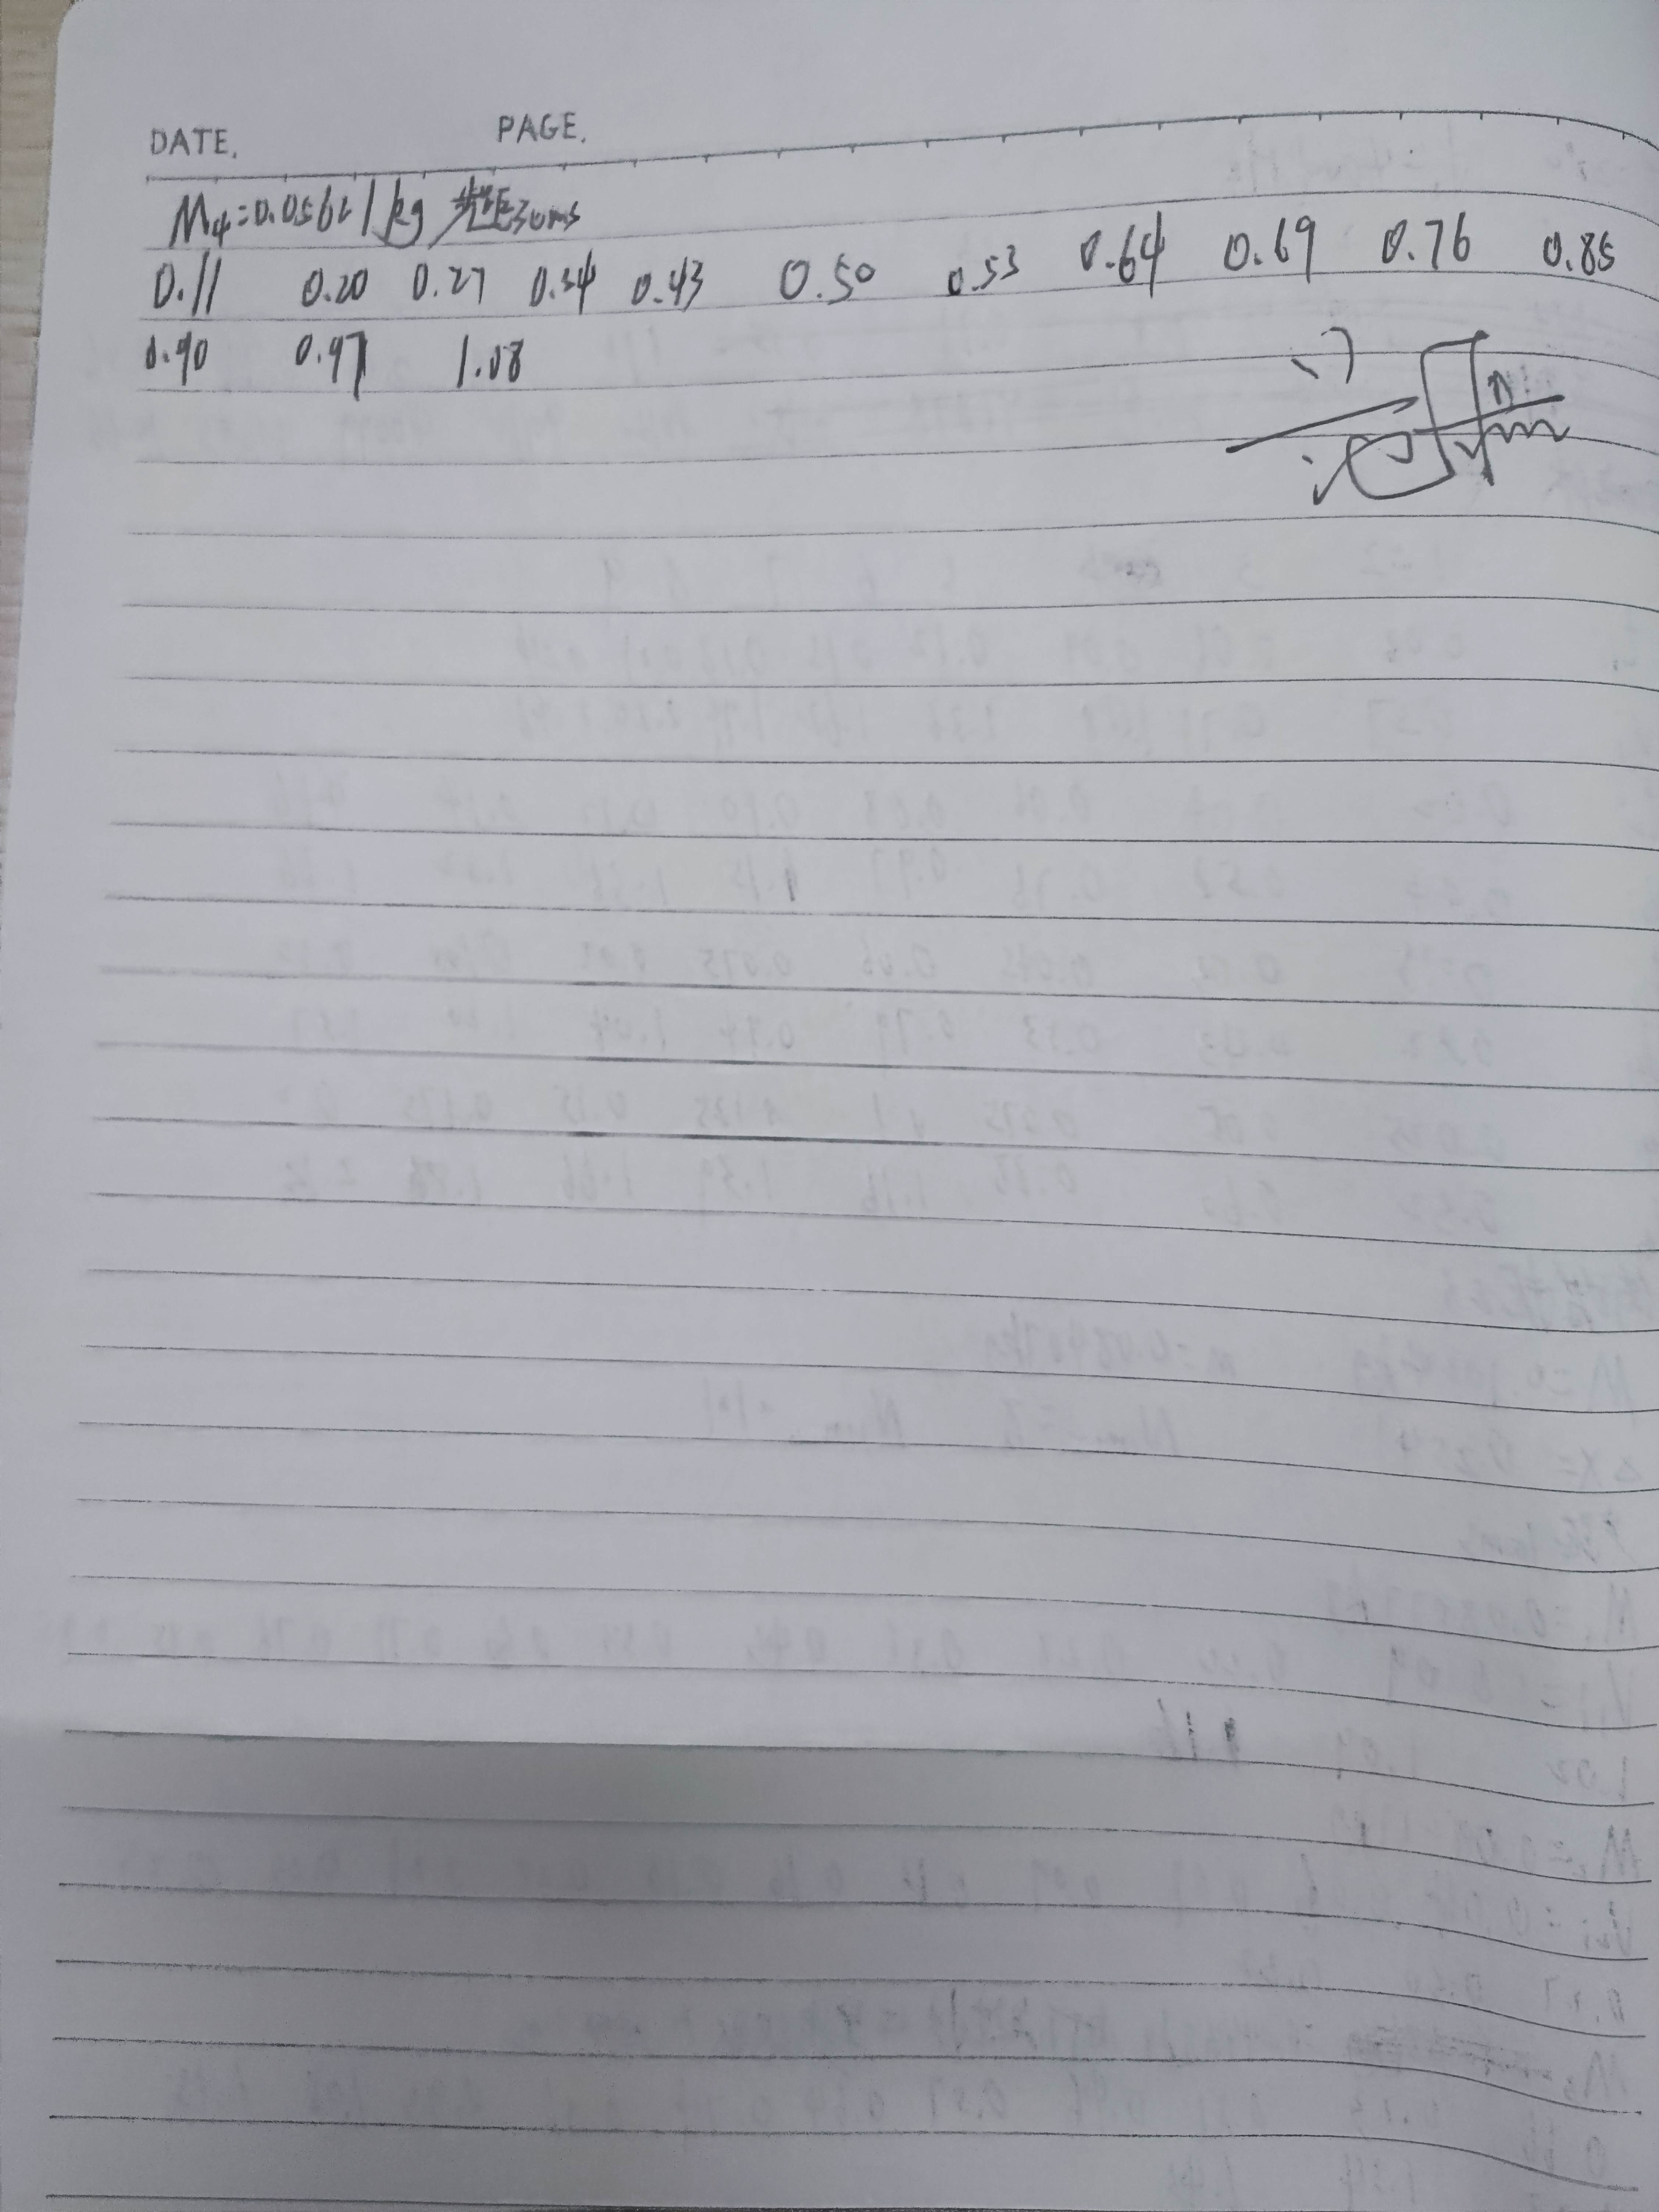
\includegraphics[width=0.4\textwidth]{多普勒原件2.jpg}
\end{figure}
\subsection*{桌面}
\begin{figure}[H]
	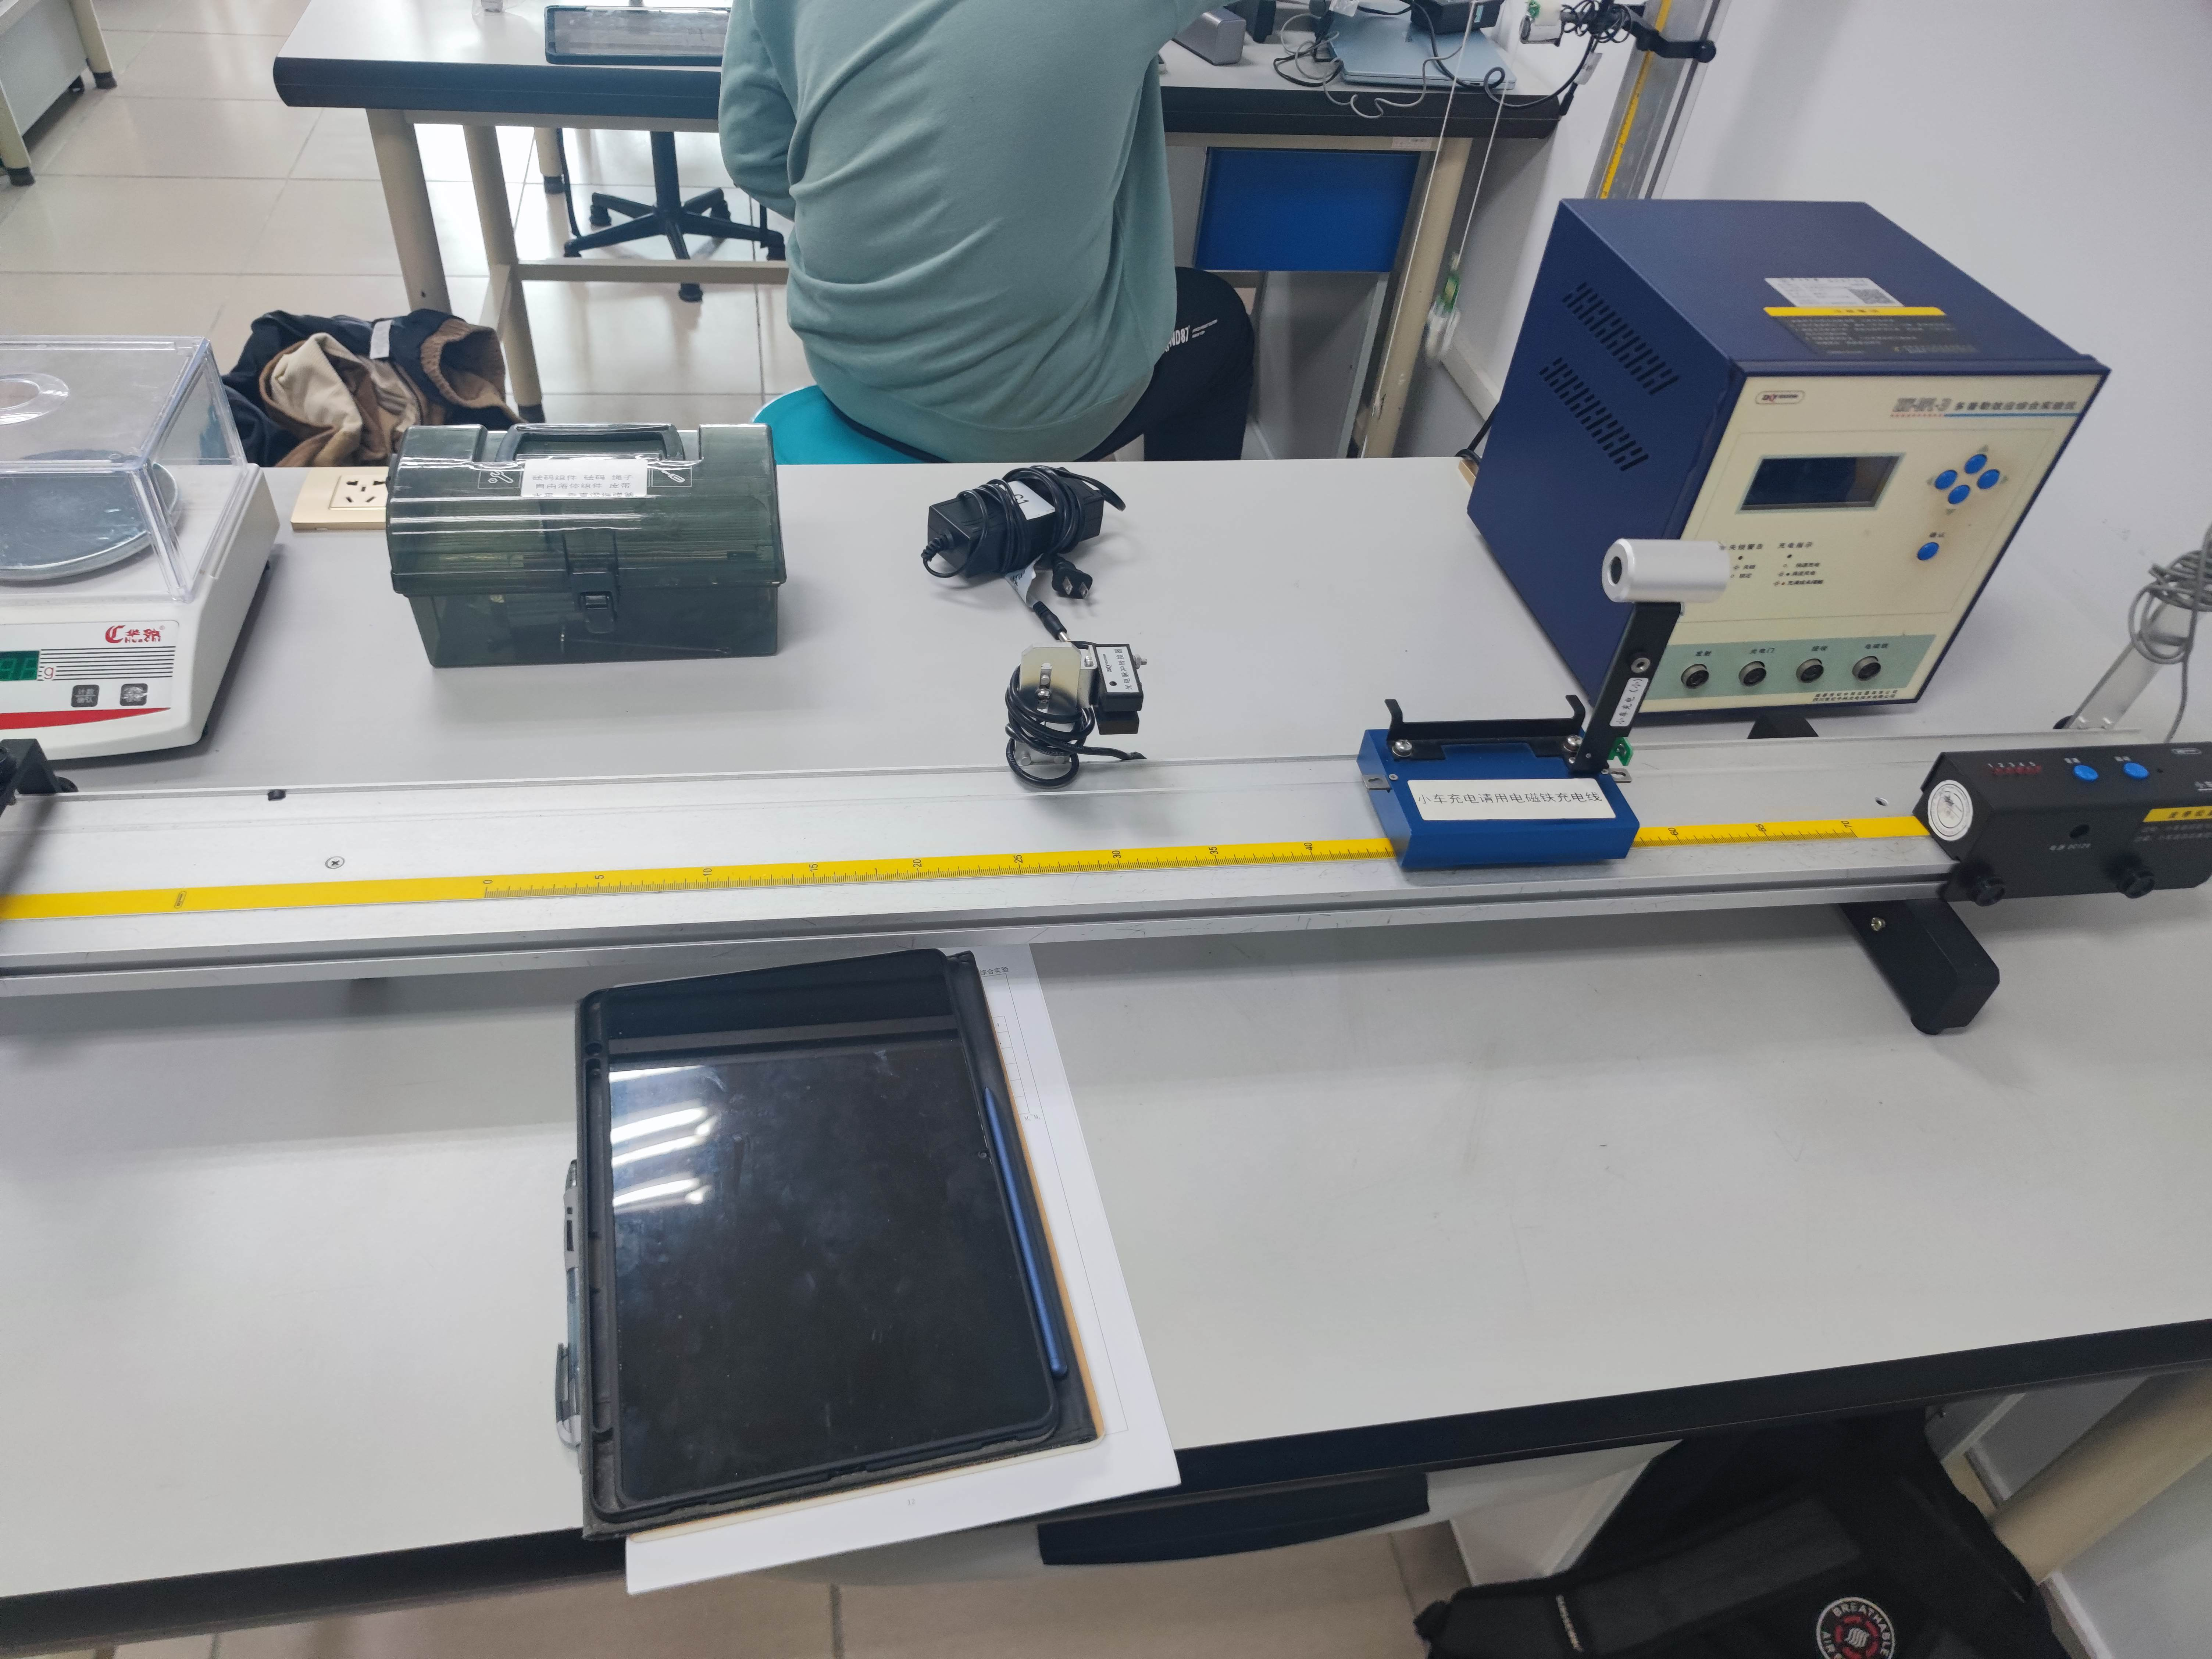
\includegraphics[width=0.95\textwidth]{多普勒桌面.jpg}
\end{figure}
\end{document}
